% main.tex - showcase of the UU beamer theme
\documentclass[aspectratio=169]{beamer}
\usetheme[showlogo]{UU}

\usepackage{amsmath}
\usepackage{graphicx}
\usepackage{physics}
\usepackage{siunitx}

% -- Metadata -----------------------------------
\title[UU Beamer Theme]{An overview of photo-current spectroscopy{\footnotesize \quad \textcolor{UUred}{v1.0.0}}}
\subtitle{To catch up Ioannis}
\author[B.J. Spijkerman]{B.J. Spijkerman}
\institute{Nanophotonics}
\date{\today}


\begin{document}
% ===========================================
%  TITLE SLIDES  (single-author, then multi-author)
% ===========================================

% -- Single-author title --
\begin{frame}[plain]
  \titlepage
\end{frame}

\begin{frame}
  \tableofcontents
\end{frame}

% ===========================================
\section{Getting Started}
% ===========================================
\begin{frame}{The principle of the measurement}
  \begin{minipage}{0.45\textwidth}
    \begin{align*}
      C_{\text{e}}&=\int_0^{\infty}d\varepsilon\,\varepsilon g(\varepsilon)\pdv[]{}{T_{\text{e}}}f(\varepsilon,T_{\text{e}})\\
      \Delta T_{\text{tot}}&=\Delta T_1 + \Delta T_2 + C\\
      \Delta\sigma&=\Delta\mu\Delta N\\
    \end{align*}
  \end{minipage}\hfill
  \begin{minipage}{0.45\textwidth}
    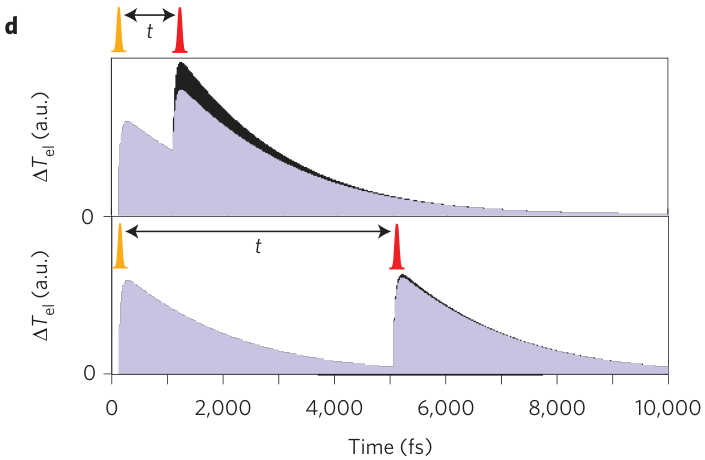
\includegraphics[width=7cm]{img/TempResponseTielrooij.png}
  \end{minipage}
\end{frame}

\begin{frame}{Optical setup}
  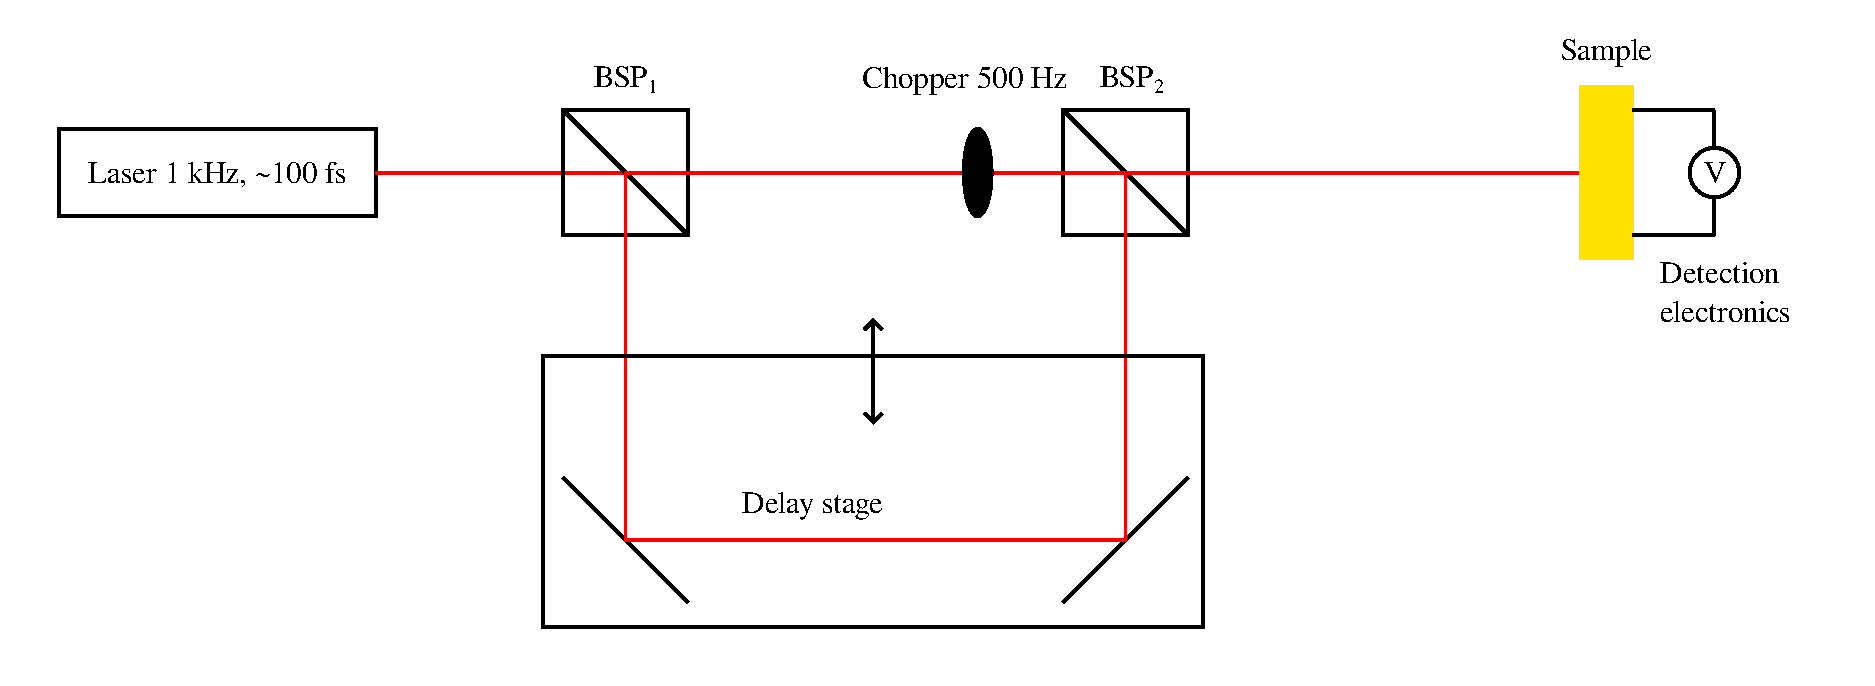
\includegraphics[width=\textwidth]{img/setup.pdf}
\end{frame}

\section{Two Temperature Model}
\begin{frame}{Two temperature model}
  \begin{align*}
    C_{\text{e}}(T_{\text{ph}})\pdv[]{T_{\text{e}}}{t}&=g(T_{\text{e}})\left(T_{\text{ph}}-T_{\text{e}}\right)+S(t)\\
    C_{\text{ph}}(T_{\text{ph}})\pdv[]{T_{\text{ph}}}{t}&=g(T_{\text{ph}})\left(T_{\text{e}}-T_{\text{ph}}\right)
  \end{align*}
  \begin{center}
    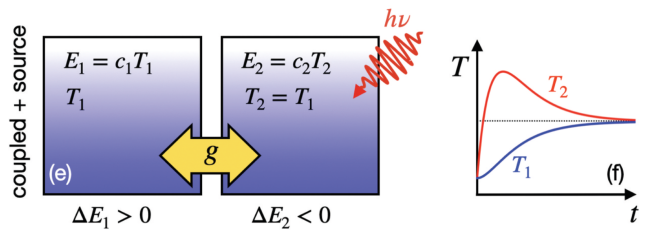
\includegraphics[width=8cm]{img/TTM_schematic.png}
  \end{center}
\end{frame}

\begin{frame}{TTM results}
  Results under a fluence of $178.254\,\unit{\micro\joule\per\square\centi\metre}$
  \begin{center}
    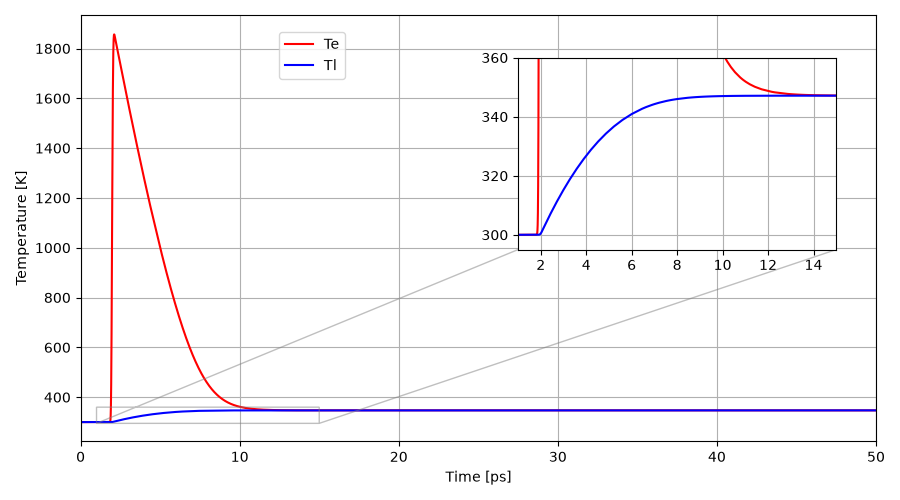
\includegraphics[width=0.8\textwidth]{img/TTMresult_adjusted.png}
  \end{center}
\end{frame}

\begin{frame}{Resistivity}
  Scattering rate $\nu_{\text{tot}}=AT_{\text{ph}}$, with $A=0.084/300\,\unit{\per\femto\second\kelvin}$
  \begin{center}
    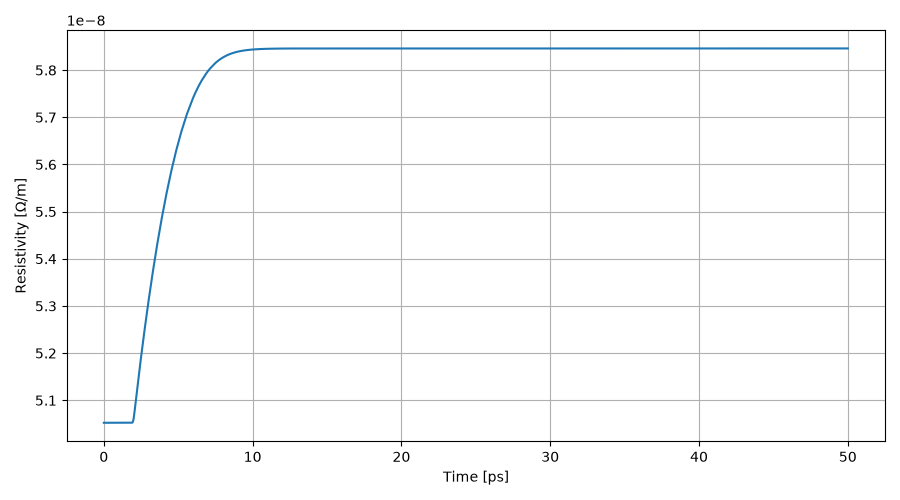
\includegraphics[width=0.8\textwidth]{img/TTMresultResistivity_adjusted.png}
  \end{center}
\end{frame}

\section{Electrical Detection}

\begin{frame}{4-point measurement}
  \begin{minipage}{0.45\textwidth}
    \begin{align*}
      V_{\text{A-B}}&=I_{\text{bias}}d\Delta\rho\\
      &=\left(100\,\unit{\milli\ampere}\right)\cdot\left(1\,\unit{\milli\metre}\right)\cdot\left(80\,\unit{\nano\ohm}\right)=8\,\unit{\pico\volt}
    \end{align*}
  \end{minipage}\hfill
  \begin{minipage}{0.45\textwidth}
    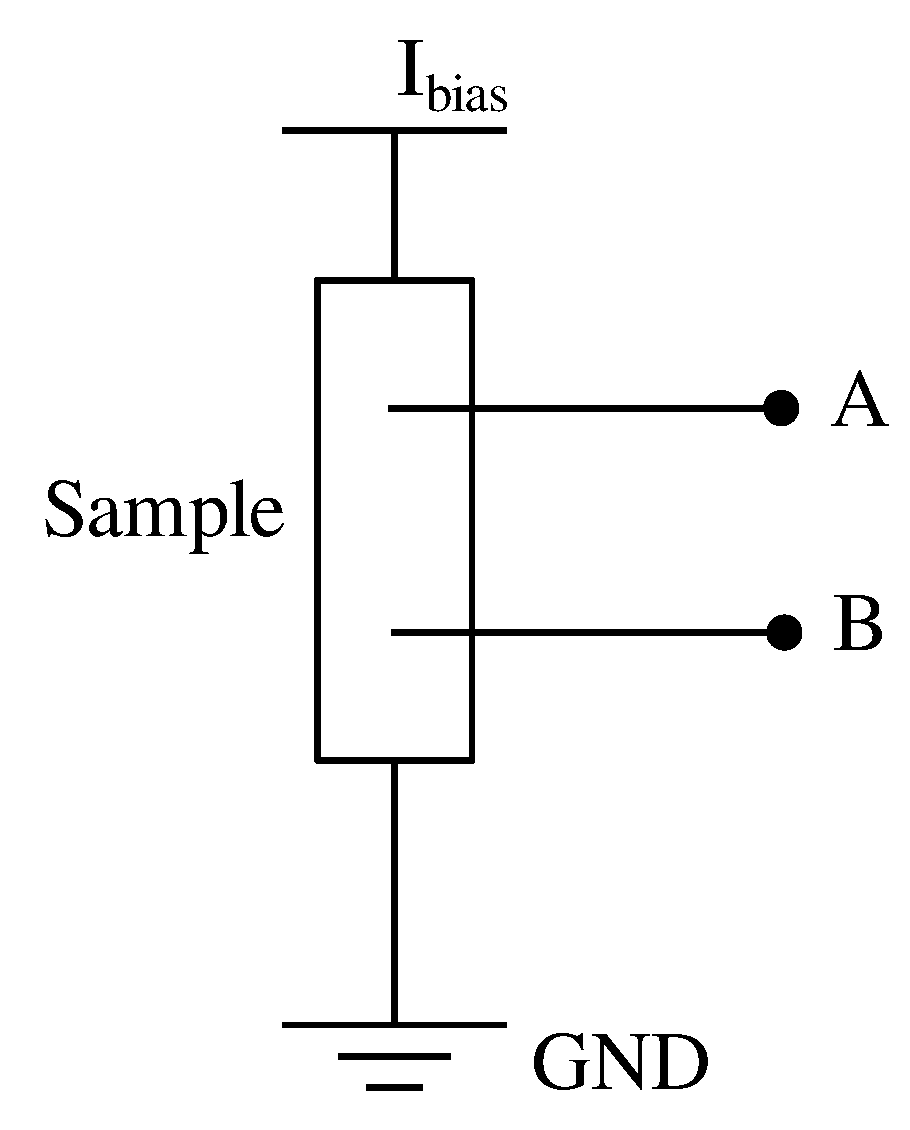
\includegraphics[height=\textwidth]{img/4-pointMeasurement.pdf}
  \end{minipage}
\end{frame}

\begin{frame}{Direct current measurement}
  \begin{minipage}{0.45\textwidth}
    \begin{align*}
      I = \frac{V_{\text{bias}}}{R_{\text{c}}+R_{\text{sample}}}
    \end{align*}
    now with $R_{\text{sample}}<<R_{\text{c}}$,
    \begin{equation*}
      I \approx V_{\text{bias}}/R_{\text{c}}
    \end{equation*}
  \end{minipage}\hfill
  \begin{minipage}{0.45\textwidth}
    \begin{center}
      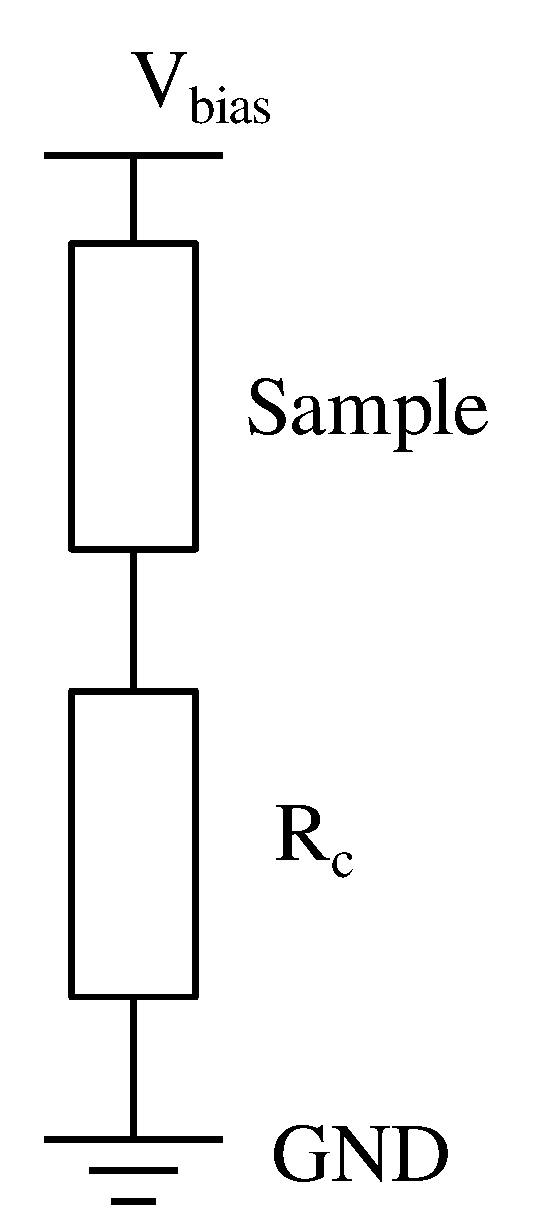
\includegraphics[height=\textwidth]{img/directCurrentMeasurement.pdf}
    \end{center}
  \end{minipage}
\end{frame}
\end{document}
